\label{user-profile}
\subsubsection{Purpose}
Any subscribed user can view or update his profile information.

The system allows taxi drivers to use the service only if they load a valid license. A reminder e-mail is sent to the taxi driver three months before the expiration.


\subsubsection{Scenario 1}
Alice, a myTaxiService passenger without a car, wants to count how many times she has used a taxi in the last month.
She opens the home page of myTaxiService page on the web site and clicks on ``login''.
After she has logged in correctly, she clicks on ``load profile'' and all the information about her account appears on screen, including the taxi request list.

\subsubsection{Scenario 2}
Gabriele's girlfriend has discovered his password but he doesn't want her to know where he has been. So he decides to change his password immediately. He opens the app on her cell phone, he selects ``load profile'' and after he selects ``modify password''. The system asks him to enter the old password and the new one two times to avoid errors. Once he has verified that everything's ok, he selects ``done'', and the system confirms that the password has been successfully set.

\subsubsection{Scenario 3}
A recall mail is sent to Bob, a myTaxiService user that has registered as taxi-driver, to notice him that he has to update his profile with a valid license. A week later he opens the app on his cell phone, he selects ``load profile'', then ``modify''. He enters the new license, then confirms selecting ``done''. The system confirms that the license has been successfully inserted.



\subsubsection{Use case}

The use case of profile management is illustrated in~\autoref{fig:usecase-profile}.
\begin{figure}
\begin{center}
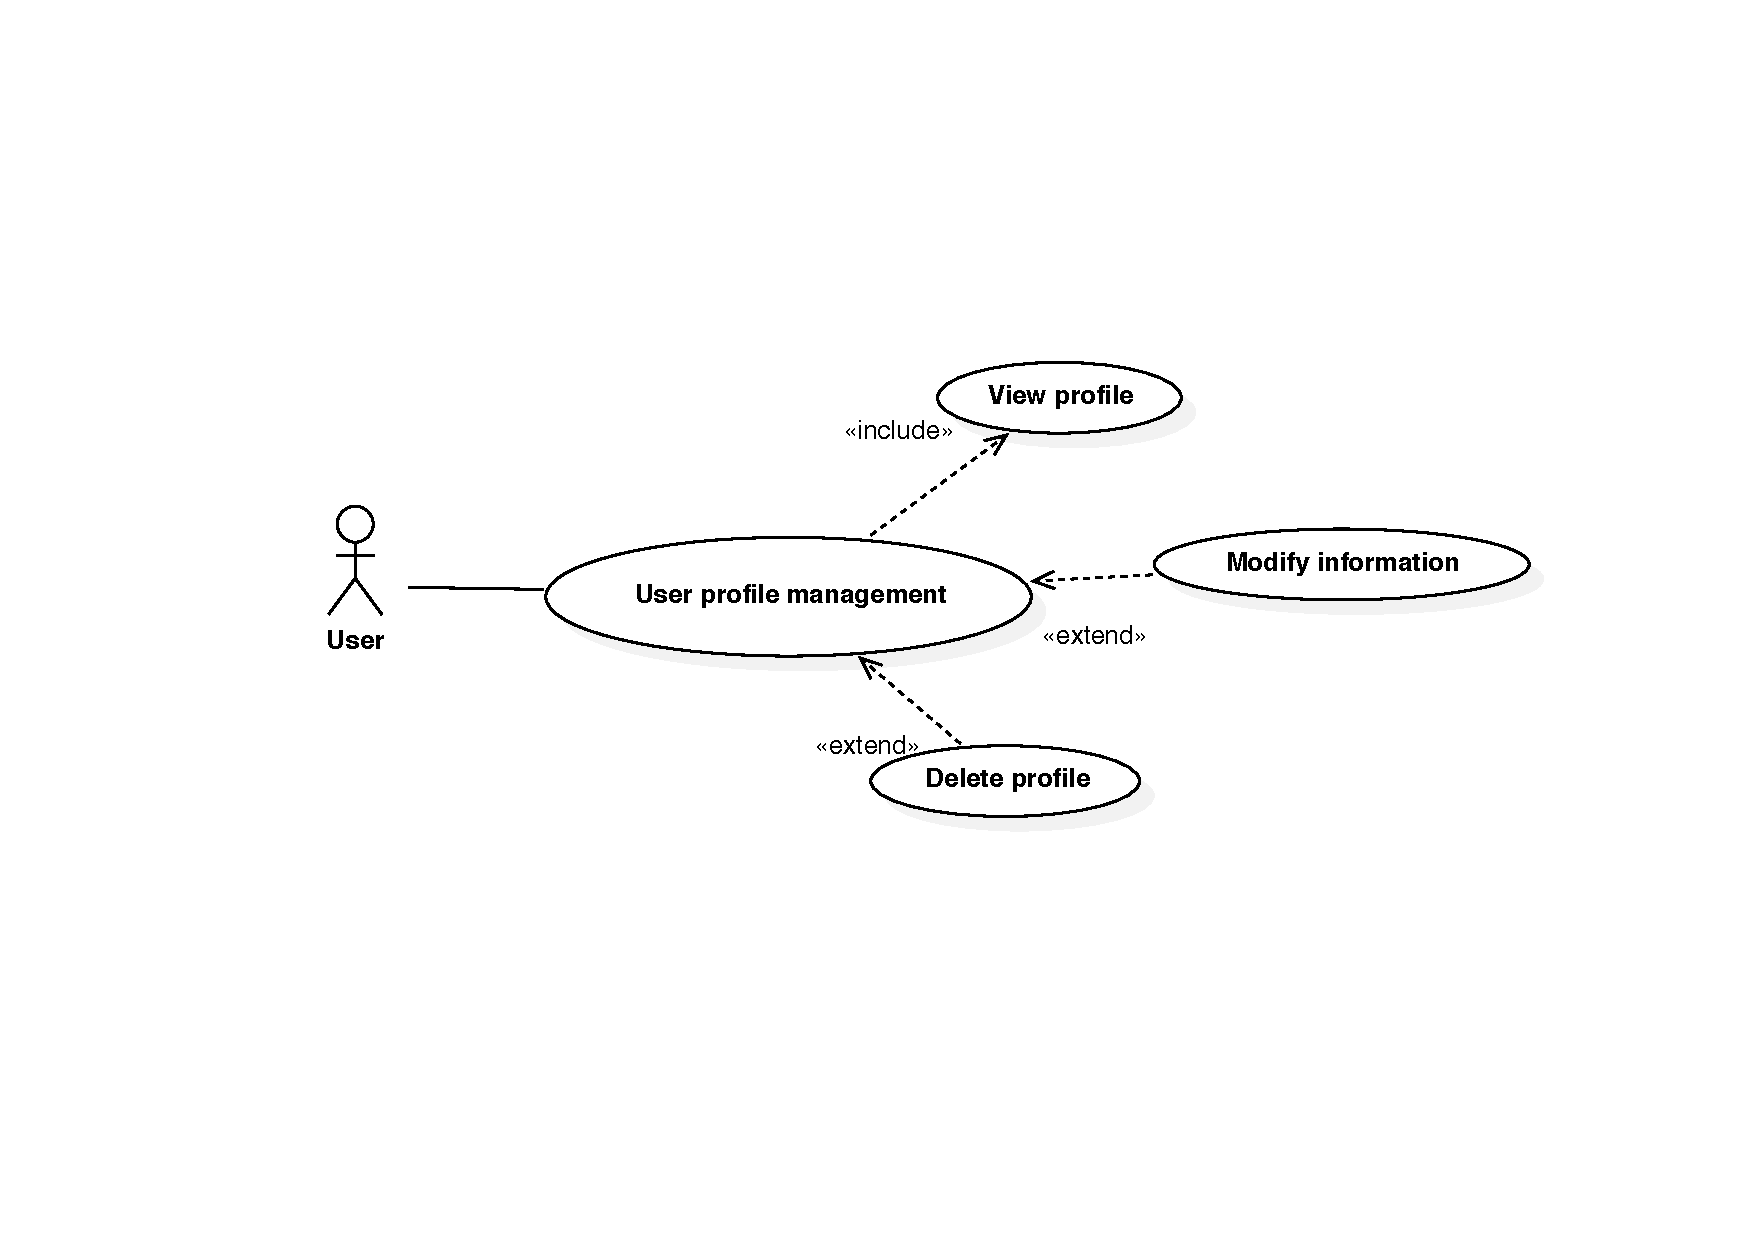
\includegraphics[width=0.7\textwidth]{diagrams/usecase_profile.pdf}
\caption{Use case diagram of user profile management.}
\label{fig:usecase-profile}
\end{center}
\end{figure}

The use case for viewing user profile is shown in~\autoref{usecase-profile-view}.

\begin{table}
\begin{center}
\begin{tabular}{| l | p{0.6\textwidth} |}
\hline
Actor & Registered user \\
\hline
Goal & Goal ~\ref{g-profile}
\\
\hline
Input condition & Passenger is already logged in and wants to check his profile.  \\
\hline
Event Flow & \begin{enumerate}
	\item The user selects load profile.
	\item The user's profile page is loaded.
	\end{enumerate}
\\
\hline
Output condition & The profile page is shown and the user can check his information. \\
\hline

Exception & None. \\
\hline
\end{tabular}
\end{center}
\caption{Use case for user profile visualization.}
\label{usecase-profile-view}
\end{table}



The use case for modifying the user profile is shown in~\autoref{usecase-profile-modify}.

\begin{table}
\begin{center}
\begin{tabular}{| l | p{0.6\textwidth} |}
\hline
Actor & Registered user \\
\hline
Goal & Goal ~\ref{g-profile}
\\
\hline
Input condition & Passenger is already logged in and wants to modify his profile.  \\
\hline
Event Flow & \begin{enumerate}
	\item The user selects load profile.
	\item The user's profile page is loaded.
	\item The user selects edit profile.
	\item The edit profile page is loaded.
	\item The user enters the new info.
	\item The user confirms
	\end{enumerate}
\\
\hline
Output condition & The information in the profile are updated. \\
\hline

Exception & If one of these requirements is not respected an exception occur:
\ref{f-modify-usrn1},
\ref{f-modify-usrn2},
\ref{f-modify-mail1},
\ref{f-modify-mail2},
\ref{f-modify-pswd1},
\ref{f-modify-pswd2},
\ref{f-modify-pswd3}.

The exception is handled ignoring the modified info, noticing the user and reloading the edit profile page. \\
\hline
\end{tabular}
\end{center}
\caption{Use case for user profile modification.}
\label{usecase-profile-modify}
\end{table}


The use case for deleting the user profile is shown in~\autoref{usecase-profile-delete}.

\begin{table}
\begin{center}
\begin{tabular}{| l | p{0.6\textwidth} |}
\hline
Actor & Registered user \\
\hline
Goal & Goal ~\ref{g-profile}
\\
\hline
Input condition & Passenger is already logged in and wants to delete his profile.  \\
\hline
Event Flow & \begin{enumerate}
	\item The user selects load profile.
	\item The user selects edit profile.
	\item The user selects delete profile.
	\item The systems asks the password.
	\item The user enters the password and confirms.
	\end{enumerate}
\\
\hline
Output condition & The user account is removed from the system database. \\
\hline

Exception & If the password entered is wrong, the user gets redirected to the ``edit profile'' page. \\
\hline
\end{tabular}
\end{center}
\caption{Use case for user profile deletion.}
\label{usecase-profile-delete}
\end{table}

\subsubsection{Associated functional requirements}
\begin{enumerate}

\item Logged passengers can:
\begin{itemize}
\item view user profile
\item modify an information
\item delete account
\item view the latest taxi request
\item view taxi requests list
\end{itemize}

\item Logged taxi drivers can:
\begin{itemize}
\item view user profile
\item modify an information
\item delete account
\item view the latest taxi request accepted
\item view requests accepted list
\end{itemize}

\item The system sends a recall mail three months before the expiration of the license submitted.

\item Delete the account:
\begin{enumerate}
\item The system allows to delete the user's account with an option on screen.
\item After ``delete account'' is selected, the user has to ensures his decision selecting on screen ``proceed'': the system deletes the account only after user's confirmation.
\item When an account is deleted all the relative information is destroyed.
\end{enumerate}

\item Modify the profile:
\begin{enumerate}
\item The system allows to change one or more information on the profile: any information can be changed, even the username or e-mail.
\item The system must verify that the new username entered is unique, i.e. there mustn't be another user that has already entered the same username.  \label{f-modify-usrn1}
\item  The system accept the new username only if it matches the regular expression\\``\texttt{[a-zA-Z][a-zA-Z0-9]\{2,20\}}''   \label{f-modify-usrn2}
\item The system must verify that the new e-mail entered is unique, i.e. there mustn't be another user that has already entered the same e-mail.   \label{f-modify-mail1}
\item If the e-mail is changed the system sends a confirmation mail on the new address.
\item The system saves the new mail only when the user clicks the link on the e-mail sent.   \label{f-modify-mail2}
\item The system accepts a new password that contains al least one number and one capital letter and that has a minimum length of eight characters.   \label{f-modify-pswd1}
\item The system accept a new password only if the old one has been submitted correctly before.  \label{f-modify-pswd2}
\item The system asks for the new password two times, when a user wants to change it.
\item The system accepts the new password only if the same one was entered twice.  \label{f-modify-pswd3}
\item The system must allow the user to abort the modification at any time.
\item The old information isn't  replaced until the ``done'' choice isn't selected by the user.
\end{enumerate}




\end{enumerate}
